\chapter{Discussion}

We have shown that our approach is capable of generally improving F1-scores in Widar 3.0, but our overall performance is disappointing, compared to both baselines and state-of-the-art approaches.
In this chapter, we discuss the experimental results and what these results mean with respect to our research questions, analyze the latent space and domain embeddings produced by our approach, as well as suggest future research that may be taken.

\section{Research questions}

In this section, we answer each of the research questions we posited in Section \ref{sec:intro-problem-statement} as well as a short discussion on the strengths and limitations of our approach to answering these questions.

\paragraph{Research Question 1}
Our first question asks how well DARLInG's embed heads perform compared to its null heads.
The results from Section \ref{sec:experiments-setup-results} show that using an RL agent indeed has the potential to increase out-of-domain performance by up to 6.2 percentage points but may also provide no benefit.
Using MTF as the transform, DDPG as the RL agent, and one-hot encoding as the domain embedding encoding provides our best results, but its low performance with the two other transforms suggest that this may not always be the case.
As such, we can conclude that while not very satisfying, our results suggest that using RL to provide unsupervised domain labels \textit{may} provide better out-of-domain performance on Widar 3.0.

\paragraph{Research Question 2}
Our second question asks how changing the domain embedding encoding affects performance.
Generally, we see inconclusive results with both encodings providing no meaningful difference generally while providing some difference with DDPG with MTF and RP transforms.
Even in these two cases, though, the difference is inconclusive as MTF prefers one-hot encoding while RP prefers probability measure encoding.
As a result, we believe that the domain embedding is not significant and that other factors contribute more towards the performance of the model.
Further research may be necessary to investigate the optimal encoding of the domain embedding.

\paragraph{Research Question 3}
Our last research question asks how changing the signal-to-image transformation affects performance.
Our results indicate that generally, GAF performs consistently, but not impressively.
MTF seems to perform quite well with DDPG and similarly to GAF with PPO.
RP seems to perform poorly with PPO, not improving over the null head, while performing similarly to MTF with DDPG.
As a result, we can confidently conclude that different signal-to-image transformations affect model performance, but the results are inconclusive as to which transformation works best.
The results do suggest, though, that MTF may be the best performer in our experiments of limited sample size.

\paragraph{Strengths and Limitations}
We believe that our experiments are quite thorough with significant resources put into ensuring that the model itself is working appropriately, as well as that the code is free of any significant bugs which could render the results invalid.
Significant effort was put into ensuring that every step of the CSI processing and transformation pipeline produced the correct results during the course of writing the thesis.
The VAE was also checked by running the VAE with the Fashion-MNIST dataset \cite{xiao2017fashion}.
This produced results as expected with the VAE being able to adequately reconstruct the input images as well as classify the images appropriately with $>0.85$ accuracy, matching the benchmarks in \cite{xiao2017fashion}.
Finally, the RL algorithms used are off-the-shelf implementations from stable-baselines3 implemented according to the sample code provided, reducing the likelihood of programmatic issues with the RL algorithms.

Limitations include reduced hyperparameter tuning and the reduced training time of the RL agents.
RL agents are notoriously time-consuming to train \cite{schulman2017proximal,schulman2017trust,lillicrap2015continuous}.
With our limited compute resources, namely a laptop and a PC, we were unable to conduct a full hyperparameter optimization sweep of the RL agents.
We mostly used known good hyperparameters when dealing with a continuous action space for our agents.
Additionally, we were only able to train for a fraction of the time usually used to train RL agents.
We also approached a PhD candidate at the TU/e specializing in RL who concurred with our ideas on the alternating training style, where we iterate between training the RL agent and the VAE \cite{grooten2023interview}.

\section{Latent Space and Domain Embedding analysis}

\begin{figure}
	\centering
	\begin{subfigure}{0.3\textwidth}
		\centering
		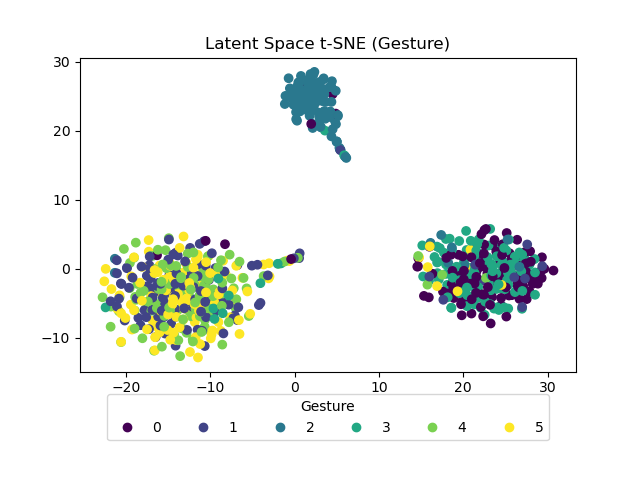
\includegraphics[width=\textwidth]{figures/mtf-ppo-one/ls-gesture}
		\caption{t-SNE by gesture}
		\label{fig:mtf-ppo-one-ls-gesture}
	\end{subfigure}
	\hfill
	\begin{subfigure}{0.3\textwidth}
		\centering
		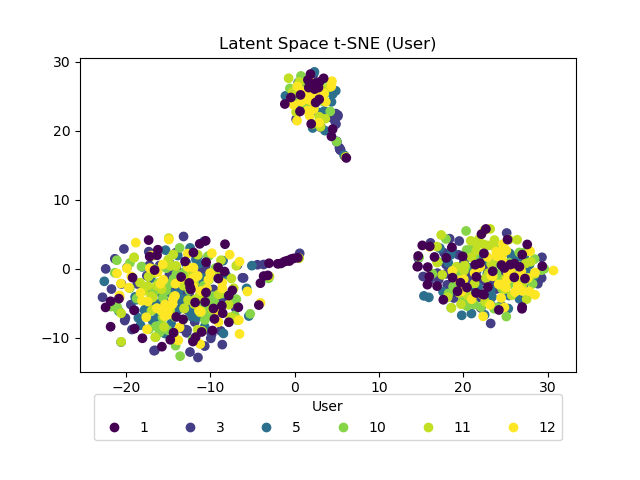
\includegraphics[width=\textwidth]{figures/mtf-ppo-one/ls-user}
		\caption{t-SNE by user}
		\label{fig:mtf-ppo-one-ls-user}
	\end{subfigure}
	\hfill
	\begin{subfigure}{0.3\textwidth}
		\centering
		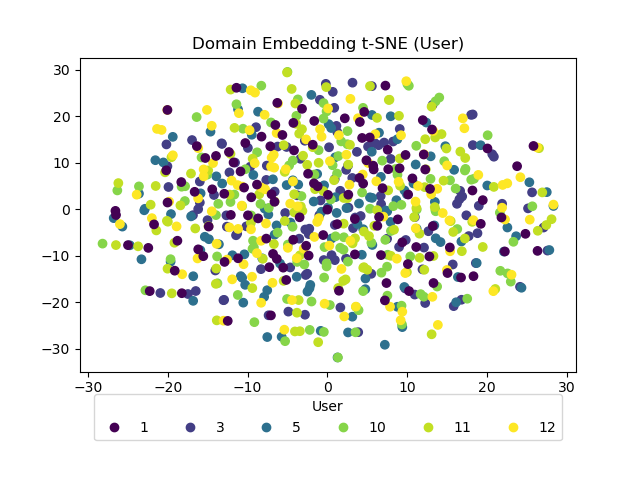
\includegraphics[width=\textwidth]{figures/mtf-ppo-one/de-user}
		\caption{t-SNE by User}
		\label{fig:mtf-ppo-one-de-user}
	\end{subfigure}
	\caption{t-SNEs of the latent space and domain embeddings produced by PPO with one-hot encoding and MTF transformation}
	\label{fig:mtf-ppo-one}
\end{figure}
\begin{figure}
	\centering
	\begin{subfigure}{0.3\textwidth}
		\centering
		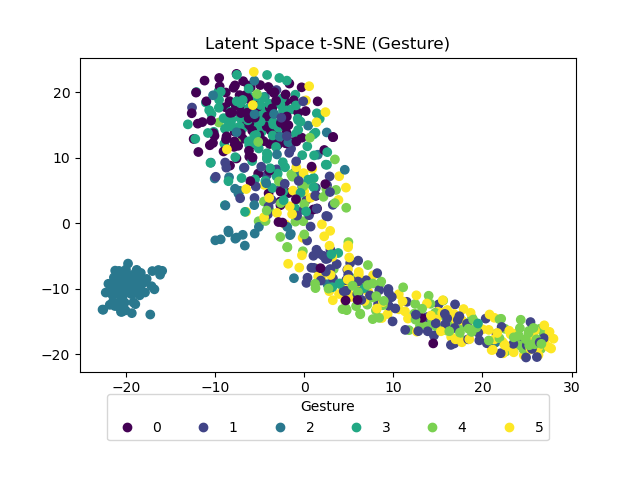
\includegraphics[width=\textwidth]{figures/mtf-ppo-pm/ls-gesture}
		\caption{t-SNE by gesture}
		\label{fig:mtf-ppo-pm-ls-gesture}
	\end{subfigure}
	\hfill
	\begin{subfigure}{0.3\textwidth}
		\centering
		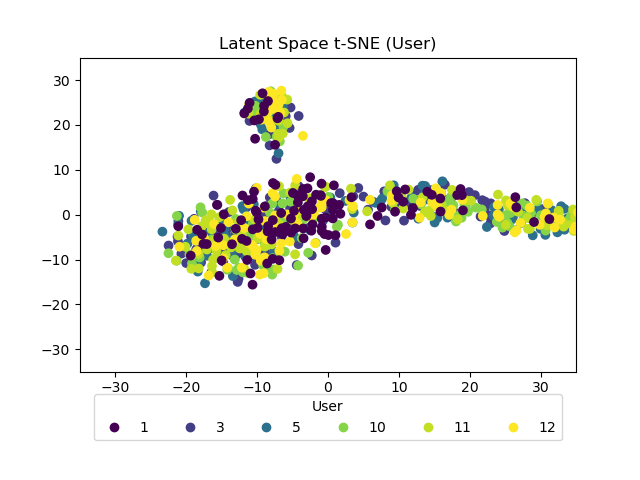
\includegraphics[width=\textwidth]{figures/mtf-ppo-pm/ls-user}
		\caption{t-SNE by user}
		\label{fig:mtf-ppo-pm-ls-user}
	\end{subfigure}
	\hfill
	\begin{subfigure}{0.3\textwidth}
		\centering
		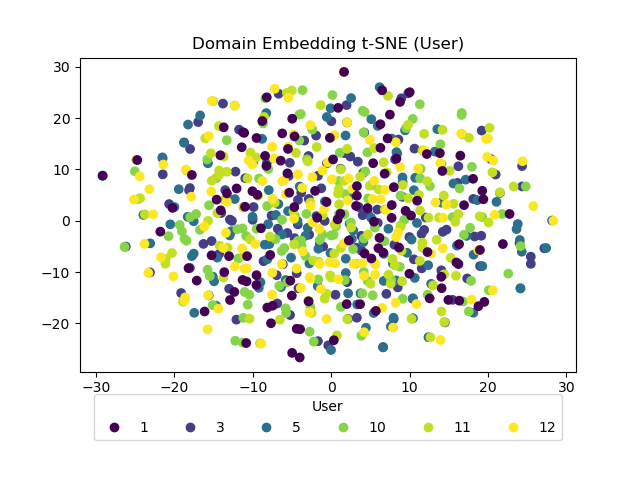
\includegraphics[width=\textwidth]{figures/mtf-ppo-pm/de-user}
		\caption{t-SNE by user}
		\label{fig:mtf-ppo-pm-de-user}
	\end{subfigure}
	\caption{t-SNEs of the latent space and domain embeddings produced by PPO with one-hot encoding and MTF transformation}
	\label{fig:mtf-ppo-pm}
\end{figure}

To properly analyze the low performance of our model, we would like to analyze both the latent space $\boldsymbol{z}$ produced by our encoder as well as the domain embeddings $\boldsymbol{d}_{r}$ produced by our RL agent.
We do this by running the entire dataset through both the encoder and RL agent and take the outputs and produce t-SNE embeddings out of these outputs.
By doing so, we can see if there is any structure to the embeddings.
We specifically analyze the case of using MTF as the signal-to-image transformation, PPO as the agent, and both the one-hot and probability measure domain embedding encodings, the results of which can be seen in Figures \ref{fig:mtf-ppo-one} and \ref{fig:mtf-ppo-pm}.

We can see that for the latent space, in both cases there is a much clearer structure, especially with gesture 2 being separated out quite distinctly in both Figures \ref{fig:mtf-ppo-one-ls-gesture} and \ref{fig:mtf-ppo-pm-ls-gesture}. 
Interestingly, both Figures \ref{fig:mtf-ppo-one-ls-user} and \ref{fig:mtf-ppo-pm-ls-user} show quite even distributions of users throughout the entire t-SNE space, indicating that the user may not significantly impact the domain embedding. \todo{t-SNE of gestures on latent space filtered by user}

For the domain embeddings, we see that there is \textit{some} structure in Figures \ref{fig:mtf-ppo-one-de-user} and \ref{fig:mtf-ppo-pm-de-user}, as it is not only a single normally-distributed disk, but there is not much of it.
We also see that the users, including the single-leave out user (user 1) is distributed quite evenly throughout the space in both figures.
This suggests that the RL agent is not able to accurately provide significantly different domain embeddings between the users.
This may be due to the latent space providing too little domain information or due to the RL agents not having been trained for enough steps but, given our current time and compute constraints, we are unable to verify either hypotheses.

\section{Future Research}

We believe that there may still be potential in our approach.
Further research could be aimed at a different neural-network architecture, hyperparameter tuning of the RL agents, and longer training times for both the VAE and the RL agents.

Although our preliminary experiments in Section \ref{sec:experiments-preliminary} suggested that our VAE model could perform adequately for the task of gesture classification with the Widar 3.0 dataset, it was evidently not up to the task of gesture classification where the input is domain shifted.
One may, instead of using a VAE, use one of the known performant models from Section \ref{sec:literature-csi-for-gesture}.
This may result in better cross-domain performance to begin with with our RL approach adding the few percentage-points on top to make said models competitive with single-domain models.

We also conducted little hyperparameter tuning of the RL agent due to time and compute constraints. 
Future research may simply repeat our experiments but with increased time and compute constraints to see if that could help at all.

Finally, we also could not train our RL agents for significant amounts of time, also due to time and compute constraints.
Future research may simply repeat our experiments with longer agent training times to see if this was the issue.
